\documentclass[varwidth=true, border=2pt]{standalone}
\usepackage{gensymb}
\usepackage{tikz}
\usetikzlibrary{arrows,positioning,decorations.pathreplacing,shapes}
\tikzset{
    %Define standard arrow tip
    >=stealth',
    % Define arrow style
    pil/.style={->,thick}
}

\begin{document}
  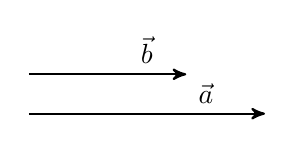
\begin{tikzpicture}
    \tikzset{
        %Define standard arrow tip
        >=stealth',
        % Define arrow style
        pil/.style={->,thick}
    }
    \draw[pil] (0,0)   -- node[near end, above] {$\vec a$} (3cm, 0cm);
    \draw[pil] (0,0.5cm) -- node[near end, above] {$\vec b$} (2cm,0.5cm);
  \end{tikzpicture}
\end{document}
